\documentclass[tikz,border=3mm]{standalone}
\usepackage{pgfplots}
\pgfplotsset{compat=1.17}
\begin{document}
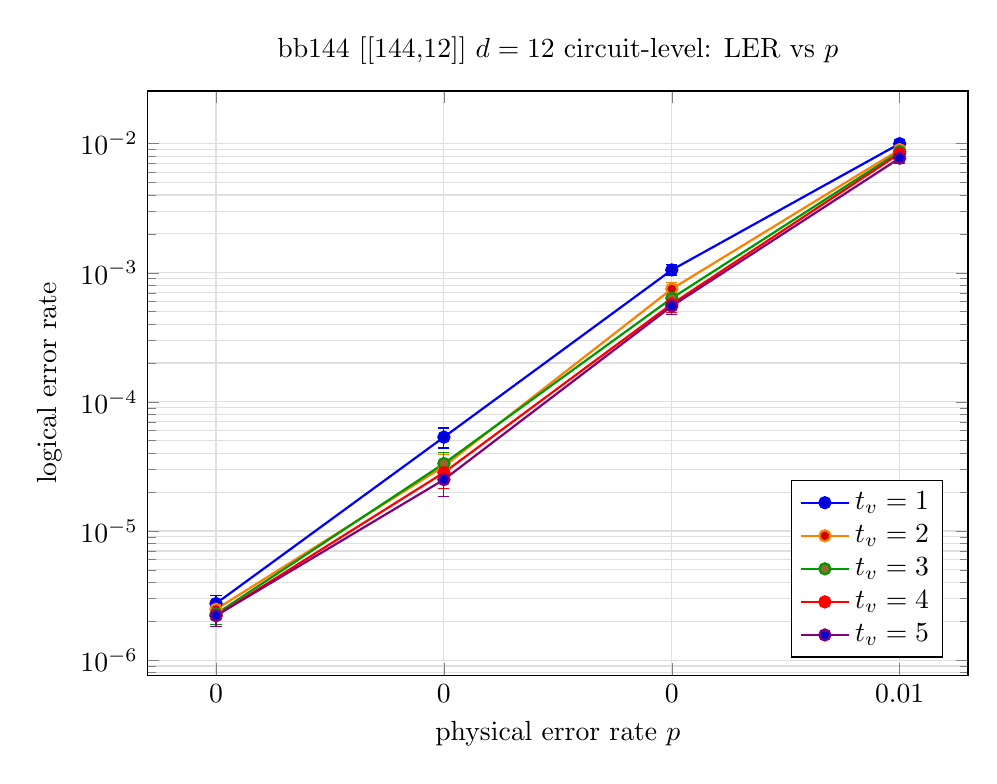
\begin{tikzpicture}
\begin{semilogyaxis}[
    width=12cm, height=9cm,
    xlabel={physical error rate $p$},
    ylabel={logical error rate},
    title={bb144 [[144,12]] $d=12$ circuit-level: LER vs $p$},
    xtick={0.002,0.003,0.004,0.005},
    scaled x ticks=false, x tick label style={/pgf/number format/fixed},
    grid=both, grid style={gray!25},
    legend pos=south east, legend cell align=left,
    mark options={solid}, every axis plot/.append style={thick},
]
\addplot+[color=blue, mark=*, error bars/.cd, y dir=both, y explicit]
    coordinates {(0.002, 2.7443e-06) +- (0, 4.2859e-07) (0.003, 5.3333e-05) +- (0, 9.4281e-06) (0.004, 1.0521e-03) +- (0, 1.0469e-04) (0.005, 1.0000e-02) +- (0, 7.4536e-04)};
\addlegendentry{$t_v=1$}
\addplot+[color=orange, mark=*, error bars/.cd, y dir=both, y explicit]
    coordinates {(0.002, 2.4766e-06) +- (0, 4.0715e-07) (0.003, 3.1667e-05) +- (0, 7.2648e-06) (0.004, 7.5000e-04) +- (0, 8.8388e-05) (0.005, 9.0000e-03) +- (0, 7.0711e-04)};
\addlegendentry{$t_v=2$}
\addplot+[color=green!60!black, mark=*, error bars/.cd, y dir=both, y explicit]
    coordinates {(0.002, 2.2758e-06) +- (0, 3.9029e-07) (0.003, 3.3333e-05) +- (0, 7.4536e-06) (0.004, 6.3542e-04) +- (0, 8.1357e-05) (0.005, 8.6667e-03) +- (0, 6.9389e-04)};
\addlegendentry{$t_v=3$}
\addplot+[color=red, mark=*, error bars/.cd, y dir=both, y explicit]
    coordinates {(0.002, 2.2088e-06) +- (0, 3.8451e-07) (0.003, 2.8333e-05) +- (0, 6.8718e-06) (0.004, 5.7292e-04) +- (0, 7.7252e-05) (0.005, 8.3889e-03) +- (0, 6.8268e-04)};
\addlegendentry{$t_v=4$}
\addplot+[color=violet, mark=*, error bars/.cd, y dir=both, y explicit]
    coordinates {(0.002, 2.2088e-06) +- (0, 3.8451e-07) (0.003, 2.5000e-05) +- (0, 6.4550e-06) (0.004, 5.5208e-04) +- (0, 7.5834e-05) (0.005, 7.7222e-03) +- (0, 6.5499e-04)};
\addlegendentry{$t_v=5$}
\end{semilogyaxis}
\end{tikzpicture}
\end{document}
